\documentclass[12pt,a4paper,oneside,final]{article}
\usepackage[utf8]{inputenc}
\usepackage[russian]{babel}
\usepackage{graphicx} % \includegraphics
\usepackage{indentfirst}

\oddsidemargin = 0cm
\topmargin = -1.5cm
\textwidth = 16cm
\textheight = 24cm
\parindent = 0.5cm

\newcommand\Section[1]{
  \refstepcounter{section}
  \section*{\raggedright
    \arabic{section}. #1}
  \addcontentsline{toc}{section}{%
    \arabic{section}. #1}
}

\newcommand\Subsection[1]{
  \refstepcounter{subsection}
  \subsection*{\raggedright
    \arabic{section}.\arabic{subsection}. #1
  }
  \addcontentsline{toc}{subsection}{%
    \arabic{section}.\arabic{subsection}. #1}
}

\newcommand\Subsubsection[1]{
  \refstepcounter{subsubsection}
  \subsubsection*{\raggedright
    \arabic{section}.\arabic{subsection}.\arabic{subsubsection}. #1
  }
  \addcontentsline{toc}{subsubsection}{%
    \arabic{section}.\arabic{subsection}.\arabic{subsubsection}. #1}
}

\sloppy

\title{Задание 2 \\
  Анализ влияния кэша на операцию матричного умножения \\
  Отчёт}
\author{Кучеров\,В.Д.}
\date{2022}

\begin{document}

\maketitle

\Section{Постановка задачи}


Реализовать последовательный алгоритм матричного умножения и оценить влияние кэша на время выполнения программы. На основе анализа влияния кэша построить графики.

\Section{Реализация}
В ходе работы подготовлено две программы: \textbf{generate\_square\_matrix} и \textbf{multiply\_matrices} для настраивомой случайной генерации квадратных матриц и перемножения матриц соответственно. Проверка корректности перемножения матриц производилось вручную с использованием стороннего ресурса - https://www.wolframalpha.com/ .Формула для умножения матриц: \\
\begin{center}
{\Large$c_{ij}=\sum_{k=1}^{n}a_{ik} \cdot b_{kj},\quad i,j = 1,2,...,n.$} \\
\end{center}

\Section{Формат командной строки}

\begin{verbatim}
./multiply_matrices <файл матрицы а> <файл матрицы b> <файл матрицы c> <режим>
\end{verbatim} 

\textbf {режим}: выбор порядка итерирования:
\begin{enumerate}
\item[0.] ijk
\item[1.] ikj
\item[2.] kij
\item[3.] jik
\item[4.] jki
\item[5.] kji
\end{enumerate}


\begin{verbatim}
./generate_square_matrix  <количество строк/столбцов> <имя выходного файла>  
                          <опц. зерно генерации> <опц. максимальное значение> 
                          <опц. генерировать отрицательные числа> 
\end{verbatim}

\begin{enumerate}
\item{\textbf{зерно генерации}:} позволяет генерировать одинаковые массивы \\
\item{\textbf{максимальное значение}:} максимальное число, которое может быть сгенерировано (по умолчанию \textbf{RAND\_MAX}) \\
\item{\textbf{генерировать отрицательные числа}:} 1 (значение по умолчанию) - генерировать отрицательные числа (максимальное значние будет при этом уменьшено вдвое), 0 - запретить генерацию отрицательных чисел\\
\end{enumerate}



\Section{Спецификация системы}

\noindent
Процессор: Intel(R) Core(TM) i9-9880H CPU @ 2.30GHz \\
Число вычислительных ядер: 8 \\

\noindent

\Section{Результаты выполнения}

Для каждого из трех размеров массивов: 300x300, 500x500, 1000x1000, было сгенерировано по 3 пары массивов A и B. В следующей таблице приведены результаты экспериментов а также усредненное время, на основе которого построены графики. 

\begin{table}[]
\begin{tabular}{|l|l|l|l|l|l|}
\hline
\begin{tabular}[c]{@{}l@{}}Число столбцов\\ (строк)\end{tabular} & \begin{tabular}[c]{@{}l@{}}Эксперимент\\ \#1 (с)\end{tabular} & \begin{tabular}[c]{@{}l@{}}Эксперимент\\ \#2 (с)\end{tabular} & \begin{tabular}[c]{@{}l@{}}Эксперимент\\ \#3 (с)\end{tabular} & Режим & \begin{tabular}[c]{@{}l@{}}Среднее время\\ выполнения (с)\end{tabular} \\ \hline
300                                                              & 0,071216                                                      & 0,072401                                                      & 0,072674                                                      & 0     & 0,072097                                                               \\ \hline
300                                                              & 0,064550                                                      & 0,063335                                                      & 0,063873                                                      & 1     & 0,063919                                                               \\ \hline
300                                                              & 0,066884                                                      & 0,067846                                                      & 0,064548                                                      & 2     & 0,066426                                                               \\ \hline
300                                                              & 0,068089                                                      & 0,066648                                                      & 0,067320                                                       & 3     & 0,067352                                                               \\ \hline
300                                                              & 0,081457                                                      & 0,091514                                                      & 0,083747                                                      & 4     & 0,085572                                                               \\ \hline
300                                                              & 0,082703                                                      & 0,082719                                                      & 0,081299                                                      & 5     & 0,082240                                                               \\ \hline
500                                                              & 0,368359                                                      & 0,358414                                                      & 0,355634                                                      & 0     & 0,360802                                                               \\ \hline
500                                                              & 0,298366                                                      & 0,292431                                                      & 0,291401                                                      & 1     & 0,294066                                                               \\ \hline
500                                                              & 0,285522                                                      & 0,289994                                                      & 0,288419                                                      & 2     & 0,287978                                                              \\ \hline
500                                                              & 0,330431                                                      & 0,345532                                                      & 0,333796                                                      & 3     & 0,336586                                                               \\ \hline
500                                                              & 0,416627                                                      & 0,423356                                                      & 0,421623                                                      & 4     & 0,420535                                                               \\ \hline
500                                                              & 0,409092                                                      & 0,404715                                                      & 0,393707                                                      & 5     & 0,402504                                                               \\ \hline
1000                                                             & 3,143482                                                      & 3,091778                                                      & 3,081808                                                      & 0     & 3,105689                                                               \\ \hline
1000                                                             & 2,264354                                                      & 2,243885                                                      & 2,254571                                                      & 1     & 2,254270                                                               \\ \hline
1000                                                             & 2,259453                                                      & 2,299128                                                      & 2,245760                                                      & 2     & 2,268113                                                               \\ \hline
1000                                                             & 2,939474                                                      & 3,023818                                                      & 3,326973                                                      & 3     & 3,096755                                                               \\ \hline
1000                                                             & 7,092690                                                      & 7,452696                                                      & 8,099096                                                      & 4     & 7,548160                                                               \\ \hline
1000                                                             & 7,041348                                                      & 7,193850                                                      & 6,778070                                                      & 5     & 7,004422                                                               \\ \hline
\end{tabular}
\end{table}

\begin{figure}[h]
\centering
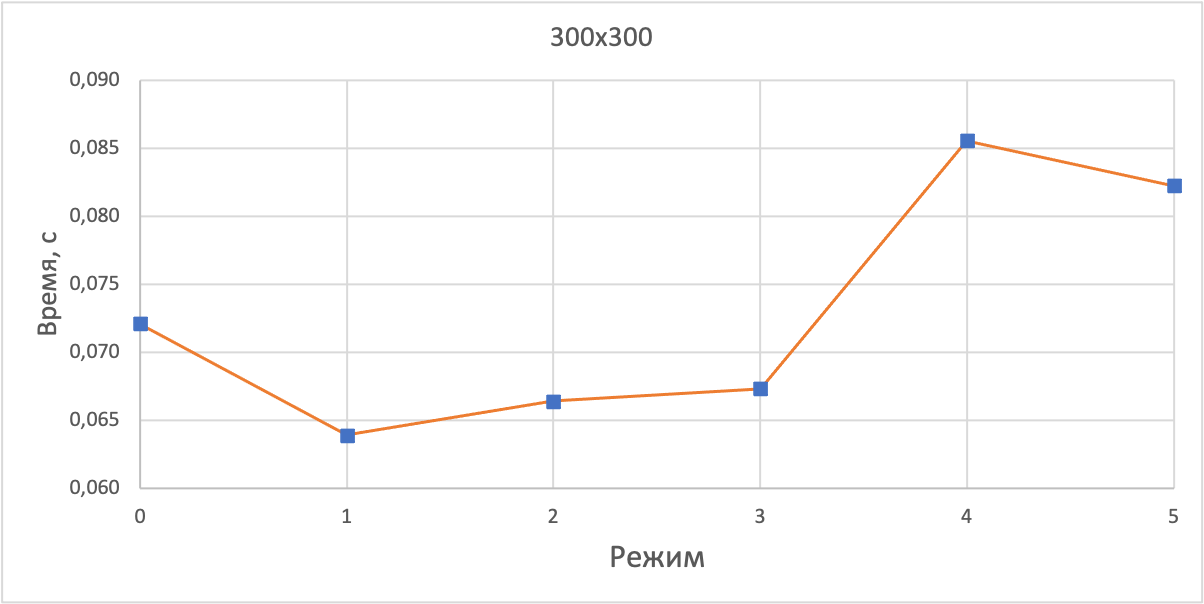
\includegraphics[width=0.8\linewidth]{300x300.png}
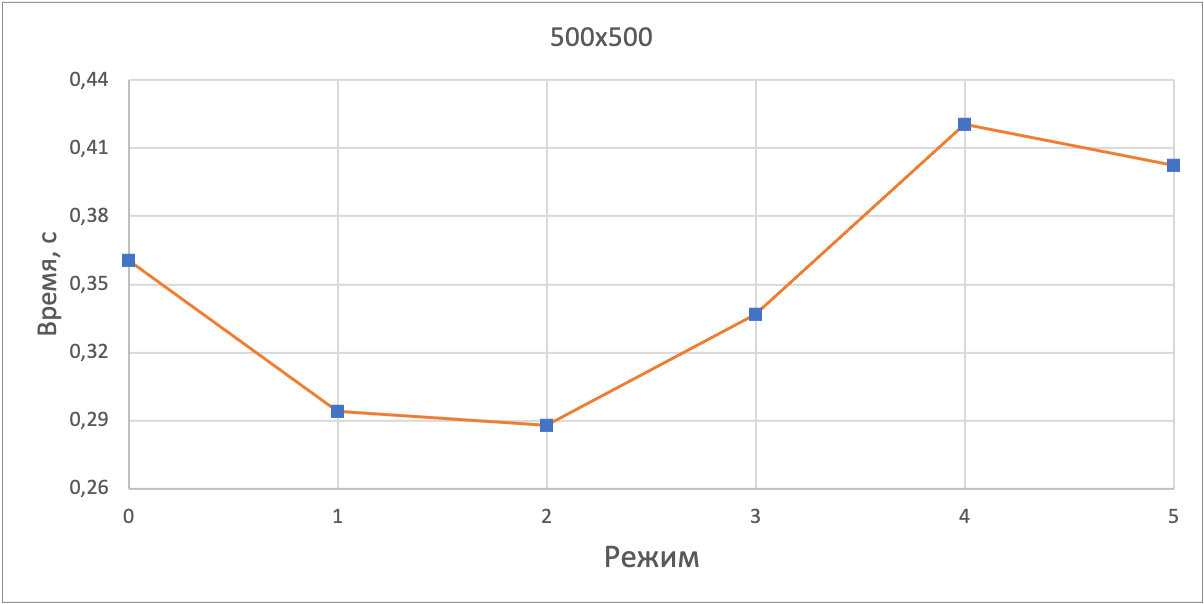
\includegraphics[width=0.8\linewidth]{500x500.png}
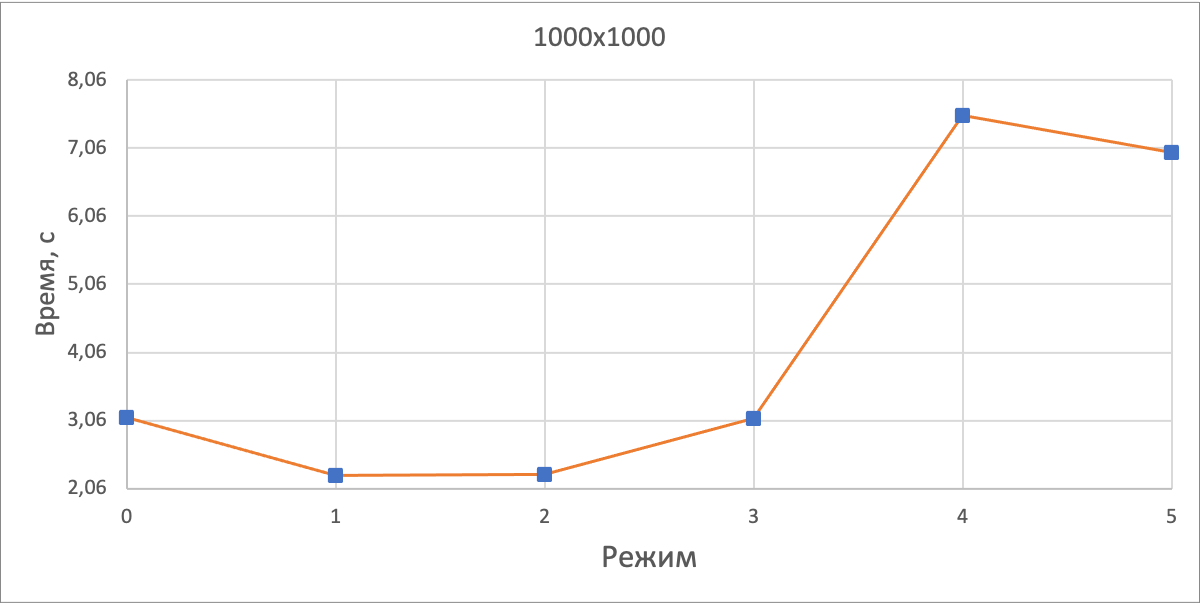
\includegraphics[width=0.8\linewidth]{1000x1000.png}
\label{fig:mpr}
\end{figure}
\end{document}
